\section{Durchführung}
\label{sec:Durchführung}
\begin{wrapfigure}{r}{0.33 \linewidth}
    \centering
    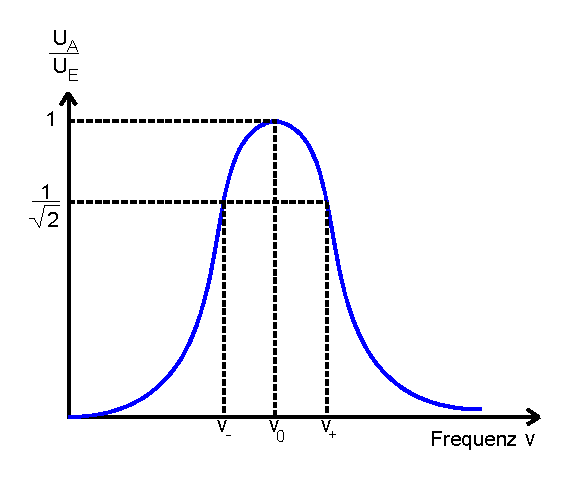
\includegraphics[width=0.8\linewidth]{pictures/Zeichnung3.pdf}
    \caption{Die Filterkurve eines Selektivverstärkers. \cite{v606}}
    \label{fig:Zeichnung3}
\end{wrapfigure}
Zunächst soll die Filterkurve, dargestellt in \autoref{fig:Zeichnung4}, des Selektivverstärkers untersucht werden.
Als Quelle wird eine konstante Eingangsspannung in Abhängigkeit von einer Frequenz gewählt.
Dafür wird als Signalquelle ein sogenannter Synthesizer gewählt.
Dieser ermöglicht eine genaue Einstellung der Frequenz.
Diese ist erforderlich um das Maximum der Filterkurve genau abzutasten.
Es wird dann jeweils die Spannung und die Frequenz notiert
Dabei wird die Güteklasse auf $Q = 20$ gestellt und die Frequenz wird im Bereich $(20 - 40) \unit{\kilo\hertz}$ eingestellt.
Nun soll weiterhin die Suszeptibilität gemessen werden.
Dafür wird der Aufbau in \autoref{fig:Zeichnung4} verwendet.
Zunächst 
Die Brückenschaltung wird so eingestellt, dass die gemessene Spannung minimal wird.
Dann wird die Einstellung am Widerstand abgelesen und notiert.
Nun wird die Probe in die Gerätschaft eingeführt und die Spannung wird abgelesen.
Schließlich wird der Widerstand so eingestellt, dass die Spannung wieder minimal wird, während die Probe eingeführt ist.
Dann wird die Probe wieder entnommen.
Im Anschluss wird dieser Prozess drei mal für jede der drei Proben wiederholt.
Während des Prozesses wird darauf geachtet, dass die Proben nicht lange in der Hand gehalten werden um diese nicht zu erwärmen
und nicht aufgrund der Temperaturabhängigkeit zwischen Messspulen und Probe die Ergebnisse zu verfälschen.

\begin{figure}
    \centering
    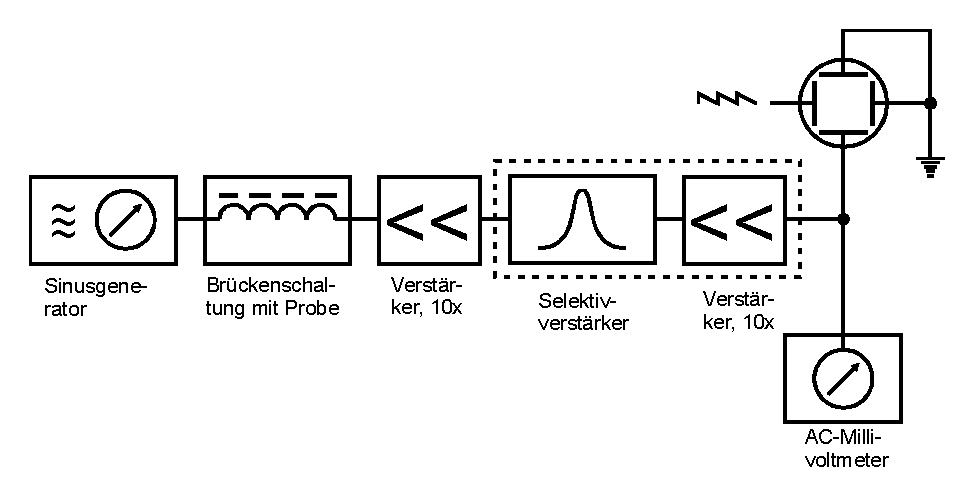
\includegraphics[width=\linewidth]{pictures/Zeichnung4.pdf}
    \caption{Blockschaltbild der verwendeten Messapparatur \cite{v606}.}
    \label{fig:Zeichnung4}
\end{figure}